% ****** Start of file apssamp.tex ******
%
%   This file is part of the APS files in the REVTeX 4.1 distribution.
%   Version 4.1r of REVTeX, August 2010
%
%   Copyright (c) 2009, 2010 The American Physical Society.
%
%   See the REVTeX 4 README file for restrictions and more information.
%
% TeX'ing this file requires that you have AMS-LaTeX 2.0 installed
% as well as the rest of the prerequisites for REVTeX 4.1
%
% See the REVTeX 4 README file
% It also requires running BibTeX. The commands are as follows:
%
%  1)  latex apssamp.tex
%  2)  bibtex apssamp
%  3)  latex apssamp.tex
%  4)  latex apssamp.tex
%
\documentclass[
reprint, amsmath,amssymb, aps,
]{revtex4-1}

\newcommand{\partDeriv}[2]{\frac{\partial #1}{\partial #2}}
\DeclareMathOperator\erf{erf}

\usepackage{graphicx}% Include figure files
\usepackage{dcolumn}% Align table columns on decimal point
\usepackage{bm}% bold math
\usepackage{hyperref}


\begin{document}

\title{On The Diffusion of Sticky Particles in 1-D}

\author{Joshua DM Hellier}
 \email{J.D.M.Hellier@sms.ed.ac.uk}
\author{Graeme J Ackland}
 \email{G.J.Ackland@ed.ac.uk}
\affiliation{
 SUPA, School of Physics and Astronomy, University of Edinburgh, Mayfield Road, Edinburgh EH9 3JZ, United Kingdom
}

\date{\today}% It is always \today, today,
             %  but any date may be explicitly specified

\begin{abstract}
The 1D Ising model is the simplest Hamiltonian-based model in statistical
mechanics. The simplest interacting particle process is the Symmetric
Exclusion Process (SEP), a  1D lattice gas of particles that hop
symmetrically and cannot overlap.  Combining the two gives a model for
sticky particle diffusion, SPM, which is described here.  SPM dynamics
are based on SEP with short-range interaction, allowing flow due to
non-equilibrium boundary conditions.  We prove that SPM is also a
detailed-balance respecting, particle-conserving,  Monte Carlo description of the Ising
model.  Neither the Ising model nor SEP have a phase transition in 1D, but the SPM exhibits a non-equilibrium transition from a
diffusing to a blocked state as stickiness increases.  We present a
fully non-linear, analytic, mean-field solution, which has a crossover
from a positive to a negative diffusion constant.  Simulations in the
positive-diffusion region agree with the analytics. The negative
diffusion constant in fact indicates a breakdown of the mean-field
approximation, with close to zero flow and breaking into a two-phase
mixture, and thus the mean field theory successfully predicts its own
demise.  The simplicity of the model suggests a wide range of
possible applications.


\end{abstract}

%\keywords{Suggested keywords}%Use showkeys class option if keyword
                              %display desired
\maketitle


\section{Introduction}

Lattice gases are a ubiquitous tool for modeling complex systems from
biology to traffic~\cite{1742-5468-2011-07-P07007, Mobilia2007,
  tegner2015high, zhu2012atomic, DealGrove1965, MottCabrera1949,
  Buzzaccaro2007}.  Analytically solvable cases involve
non-interacting or excluding particles~\cite{ladd1988application,
  liggett1985interacting, BenNaim1999, Shandarin1989, Frachebourg1999,
  Frachebourg2000}, but in any real system of interest the moving
objects interact. Many models tackle the situation where the diffusing
object interact with the substrate, but despite the clear
application-relevance there is surprisingly little work considering
interactions between the moving particles themselves.  One reason for
this is that the interactions introduce nonlinearities in analytical
models, which makes them challenging to solve, at least outside of
limits in which they can be linearized. This is unfortunate because it
is precisely these nonlinearities which introduce interesting
behaviors such as discontinuities at the oxide-metal interface or
diffusion instability~\cite{Obukhovsky2017, Gorokhova2010}.

Another feature of previous models is that the flow is driven by
either asymmetry in the dynamics (e.g. ASEP) or an external field
which permeates the system (e.g. KLS).  In either case, the particles
always see a local asymmetry.  However in many systems the flow is
driven by a pressure or chemical potential difference applied at the
boundaries, so that any local asymmetry arises from self-organization.
This situation is addressed here.

In this paper we will investigate a simple one-dimensional model, the
``Sticky Particle Model'' or SPM, specified in the top left inset of
Fig.~\ref{fig:lambdaScans}, which contains such an interaction, and we
will explore the impact this has on particle behavior, in particular
when observed in the large-scale limit.  One might contrast this
approach (making a simple microscopic model and trying to learn from
it about large-scale interface growth) with approaches such as the KPZ
equation~\cite{PhysRevLett.56.889, PhysRevA.38.4271, Sasamoto2010}
(where one analyses the extreme large-scale dynamics using
universality classes).

% \begin{figure} \vspace{1em}
%\caption{\label{fig:detailedBalance} White circles indicate particles, dark circles indicate empty sites (vacancies). Particles randomly move into adjacent vacancies with rate $1$ (having rescaled time for notational convenience), unless there is a particle behind the position they're moving from, in which case they move with rate $\lambda$; the state of the site next to the position the particle is moving into is irrelevant. Particles also move to the left, with rates such that the whole model is totally symmetric.}
%    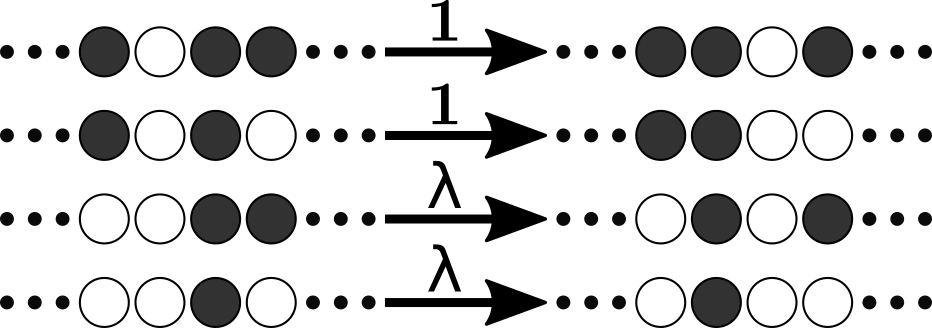
\includegraphics[width=\linewidth]{newRates.png}
%    \end{figure}


\begin{figure}[h!]
\vspace{1em}
\setbox1=\hbox{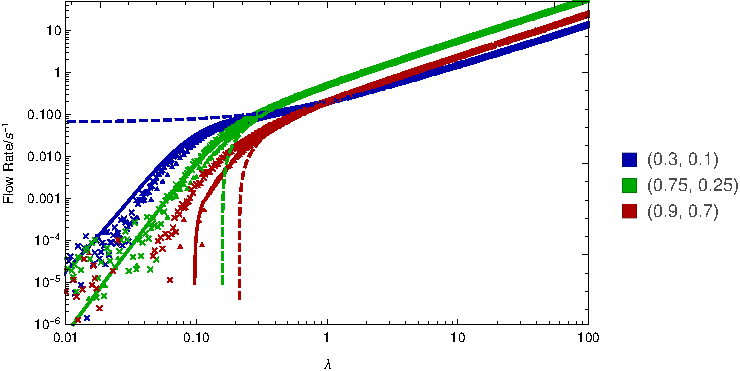
\includegraphics[width=\linewidth]{logFlowRates.pdf}}
  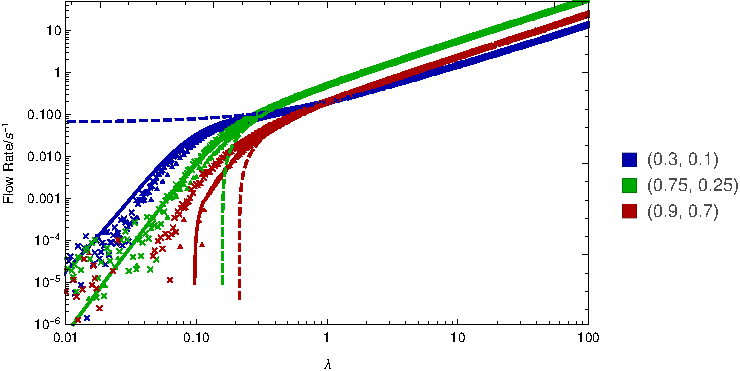
\includegraphics[width=\linewidth]{logFlowRates.pdf}\llap{\makebox[0.525\linewidth][l]{\raisebox{1.2cm}{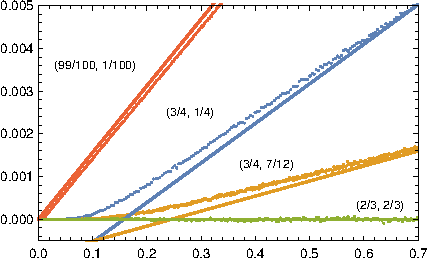
\includegraphics[width=0.475\linewidth]{linearFlowRates.pdf}}}}\llap{\makebox[0.85\linewidth][l]{\raisebox{7.75cm}{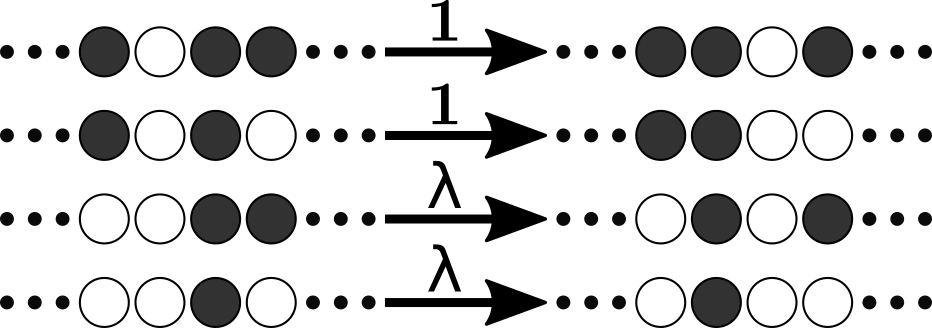
\includegraphics[width=0.45\linewidth]{newRates.png}}}}
    \vspace{-1em}
\caption{\label{fig:lambdaScans} \textbf{Top left:} White circles
  indicate particles, dark circles indicate empty sites
  (vacancies). Particles randomly move into adjacent vacancies with
  rate $1$ (having rescaled time for notational convenience), unless
  there is a particle behind the position they're moving from, in
  which case they move with rate $\lambda$; the state of the site next
  to the position the particle is moving into is irrelevant.
  Particles also move to the left, with rates such that the whole
  model is totally symmetric.\\ \textbf{Bottom right:} Mean flow rate
  observed when varying $\lambda$ with fixed boundary densities
  $(\rho_0, \rho_L)$ as labeled in the plot.  The MFT
  prediction is indicated by the solid line.  In each case we used
  systems of length $64$ (length $32$, $128$ and $256$ give similar
  results), running them for $4\times10^5$ Gillespie steps for
  equilibration followed by $10^4$ independent data gathering runs of
  $10^3$ steps, interspersed with relaxation runs of $16000$
  steps. This way we could gather statistics about flow rates and
  densities in a well-equilibrated system. Specifically, we generate a
  pool of $10000$ samples of flow rate and density from which we can
  calculate estimates of the descriptive statistics of both
  quantities; flow moments and the density data are included in the
  supplementary materials.\\ \textbf{Main figure:} As the blue $\left(
  \frac{3}{4} , \frac{1}{4} \right)$ data on the inset plot, with the
  same boundary conditions and run parameters, but with both axes
  logarithmic and over a wide range of orders of magnitude of
  $\lambda$.  The dashed lines represent power-laws; the
  higher-$\lambda$ one is asymptotically matched to the mean-field
  prediction, whilst the lower-$\lambda$ one is fitted to the
  power-law behavior in the range $0.04 \le \lambda \le 0.1$.
\vspace{1em}}
\end{figure}

\section{The sticky particle model}

The SPM is an excluded-particle model in which adjacent particles
separate with rate $\lambda$ and single particles move at rate $1$.


It differs from the symmetric exclusion
process~\cite{sugden2007dynamically, Kollmann2003, Lin2005,
  Hegde2014,Krapivsky2014, Imamura2017}; in that particles ``unstick''
with rate $\lambda$ instead of their normal hopping rate, $1$.  Low
$\lambda$ corresponds to sticky particles, high $\lambda$ to repelling
particles.
It could be regarded as a version of the KLS model~\cite{Katz1984,
  Zia2010, Kafri2003} in 1-dimension without an applied field, which
is itself similar to the dynamics used to analyze the Ising model by
Kawasaki~\cite{PhysRev.145.224}.  The KLS model has a field which
introduces an asymmetry which drives a flow.  It is tacitly assumed
that this field is required for the nontrivial flow behavior seen in
the model, so the simpler symmetric model has received less attention.


\subsection{Detailed Balance Proof} 
The SPM is intended to study flow, so it is {\it defined} by the
hopping rates.  In Fig.~\ref{fig:lambdaScans} we
show all the possible transitions which may occur between local
configurations. 

Assume that the system is now on a ring, with $L$
lattice sites and $N$ particles.  Let us label possible system
configurations by $\xi$ and let the number of adjacencies (or
``bonds'') between particles be $b(\xi)$. Now for our ansatz, assume
that the probability of the system being in state $\xi$ is
$\lambda^{-b(\xi)}$.  In the top and bottom diagrams of
Fig.~\ref{fig:lambdaScans} we can see that the number of bonds on
both sides is the same, as are the transition rates back and forth;
thus our ansatz holds for these states, as it predicts the
probabilities of the left and right configurations are the same. The
middle two diagrams are equivalent; in the upper diagram a
bond is formed going left to right and then broken going right to
left, so the probability of being in the left state is $\lambda$ times
that of being in the right state. This is again in agreement with the
detailed balance criterion. As these are the only types of transition
that may occur on a ring, we have proven that the closed system obeys
detailed balance.

\subsection{Equivalence to Ising Model at Equilibrium}

Since the model obeys detailed balance, there must be an associated
Hamiltonian.  This is simply the number of particles stuck together
\[ H = \sum_i p_ip_{i+1} \]
where $p_i$ is 1 for a particle or zero for and empty site.  A simple
transformation $s_i = 2p_i-1$ shows this to be equivalent to the Ising
Hamiltonian
\[ H = \sum_i \frac{1}{4} s_is_{i+1} + \frac{1}{2} s_i + \frac{1}{4}\]
The final term is constant, and only hopping moves are allowed so that
$\sum s_i$ is also constant. So at equilibrium the SPM samples the 1D
Ising model with fixed magnetisation, a fact which was used to
validate the codes.


\section{Simulations}

 In our system the bulk is perfectly symmetric, and flow is driven by
 setting $\rho$ at the boundaries, with the system self-organising to
 give the steady-state density. Thus the boundary concentrations,
 $\rho_0$ and $\rho_L$ are the independent variables which drive the
 system.  The flow rate, Hamiltonian energy and particle density of the system are fully determined by  $(\rho_0, \rho_L)$ and the unsticking rate $\lambda$


  We chose to calculate using the \texttt{KMCLib}\cite{leetmaa2014kmclib}
 package, which implements the Kinetic Monte Carlo algorithm
 (essentially the same as the Gillespie algorithm\cite{Gillespie1977,
   Bortz1975, Prados1997}) on lattice systems. The codes used are kept
 here~\cite{jHellGitRepo}.

We are interested in flow in a bounded domain, and can simulate that
situation using KMC. In the bulk, the transition rates are simply
those described in Fig.~\ref{fig:lambdaScans}. At the boundaries there
are 2 layers of lattice sites that switch between being full and empty
with rates such that the time-averaged occupation ($\rho_0, \rho_L$)
defines the boundary conditions; The system is therefore open, and
particles appear and disappear at boundary layers.  These boundaries
are equivalent to having particle reservoirs attached to the edges of the
domain.

Independent of the KMCLib code, we wrote a simple Metropolis-Hastings
algorithm which randomly selects single particle hops.  Except for
extreme $\lambda$s, this has an acceptance rate of order 10\%. Results
determined from the KMC and Metropolis-Hastings codes are
indistinguishable.

We calculated the flow from the number of particles entering and
leaving the system at the boundaries.  Since the model is defined in
terms of {\it rates}, the flow in ``particles per unit time'' is well
defined quantity.

In the simulation, we can vary $\rho_0$, $\rho_L$ and $\lambda$ to
address three questions: how does $\lambda$ affect the flow, how does
the flowrate depend on the driving force $(\rho_0 - \rho_L)/L$, and
how does the density of particles in the system vary.

Using KMClib we studied systems of length $64$ (length $32$ gives similar
results), running them for $400000$ Gillispie steps for equilibration
followed by $10000$ measurement runs of $1000$ steps interspersed with
relaxation runs of $16000$ steps. This way we could gather statistics
about flow rates and densities in a well-equilibrated
system. Specifically, we generate a pool of $10000$ samples of flow
rate and density, from which we can calculate estimates of the
descriptive statistics of both quantities.


\subsection{Transition in flow character}

Fig\ref{fig:lambdaScans} shows how the flowrate varies with stickiness
at fixed driving.  At high $\lambda$ the rate is simply proportional
to $\lambda$ for any forcing.  This result is far from trivial - it
means that the overall flow is determined by the {\it faster} rate
$\lambda$, not the slower rate (1).  That the MFT averages over the
two is unsurprising (Eq. \ref{eq:diffCoef}), but for the
simulation to avoid having a ``rate limiting step'' requires the
system to fill to sufficient density that there are always particles
in contact to repel one another.

At low $\lambda$ the simulation shows a transition to a different
behavior, the flow rate remains finite.  This transition corresponds
to a distinctive peak in the particle density fluctuations
$<(\rho-\bar{\rho})^2$ (Fig.\ref{fig:DenFluc}).  The width of the peak is independent of the
system size 
which suggests a continuous
phase transition from the free flowing to the ``stuck'' regime.

At very low
$\lambda$ it becomes exceptionally rare for a particle or vacancy to
traverse the whole system, the KMC is unable to generate good statistics, 
and the flow measurement is dominated by
the noise of boundary fluctuations.
However, there is a regime when $0.04 \le \lambda \le 0.1$
where the mean flow again displays clear power-law behavior, this time
with $\mathcal{O}~(\lambda^{4})$; between this region and the
$\lambda^1$ region there is a bend as we switch between the power laws.

\subsection{Effective diffusion constant}


Using boundary conditions $(\rho_0, \rho_L) = (\rho_M + \frac{1}{2}
\delta\rho, \rho_M - \frac{1}{2} \delta\rho)$ we demonstrate the
dependence of flowrate on driving and $\lambda$.  (Fig \ref{fig:constDens}).  This
shows that the transition to the stuck phase is suppressed by stronger
driving forces (large $|\delta\rho|$)

We use the limit of small $\delta\rho$ to calculate the effective
diffusion constant.  This is normalised to 1 in the case of
$\lambda=1$, which is just SEP.  The $\rho_M=0$ limit corresponds to
free flow of particles, so the diffusion constant here does to
1. Similarly the $\rho_M=1$ limit is flow of vacancies, so
$D\rightarrow\lambda$.  One might expect a monotonic variation between
these limits, but surprisingly the simulations show that there is
always an extremal value for $D$ close to $\rho_M=2/3$: this is a
minimum for $\lambda<1$ and a maximum for $\lambda>1$


\subsection{Self-organised density}


We calculated the time-averaged total number of particles in
the system by updating a histogram of particle numbers
as the simulation progresses. In each of our calculations, we make the
initial configuration by randomly filling the system with particles
and vacancies in such a way that the initial density should be
$\frac{1}{2}(\rho_0 + \rho_L)$, and then run the system for a
sufficient number of equilibration steps to destroy any initial
transients.

In SEP, ($\lambda=1$) the density varies linearly across the system
from $\rho_0$ to $\rho_L$, as one expects for a diffusion process.
However, for sticky particles, $\lambda<1$, the density rises sharply
near to the boundary, then has a linear profile about a value higher
than $\rho_M$  (Fig.\ref{fig:flowStats}d). 
One might view this as particles being sucked into the
system to lower their Hamiltonian Energy, but such a notion can be
dismissed since the internal density {\it also rises for repelling
  particles}, $\lambda>1$.  The asymptotic values for the density at
high and low $\sigma$ appear to be 1 and $\frac{2}{3}$, regardless of the 
mean boundary density $\rho_M$.
Fig \ref{fig:DenProfile} 



\begin{figure}[h!]
\vspace{1em}
\begin{center}
    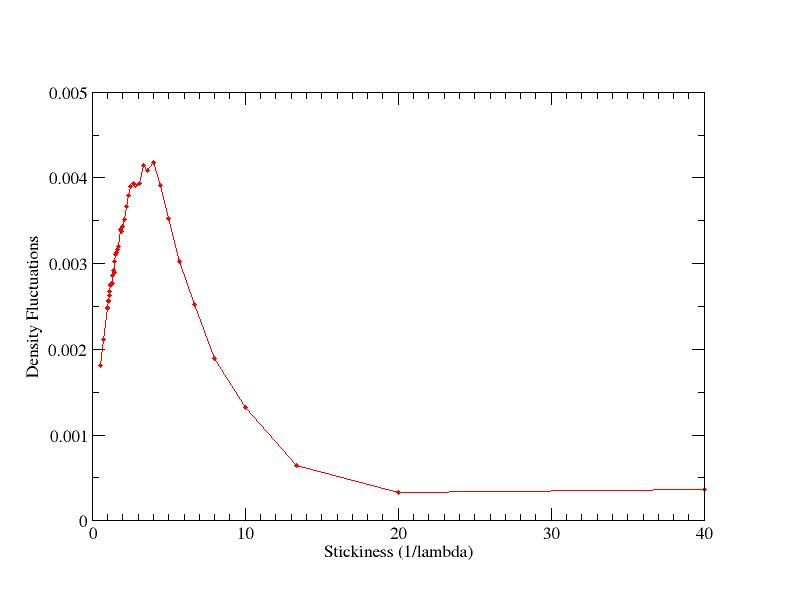
\includegraphics[width=0.5\linewidth]{densityFluct.jpg}
\end{center}
    \vspace{-0em}
\caption{\label{fig:DenFluc} [Placeholder] Density fluctuation 
as a function of $\lambda$
 for a  range of system sizes 
 with boundary conditions
  (0.6, 0.4) }
\end{figure}

\begin{figure}[h!]
\vspace{1em}
\begin{center}
    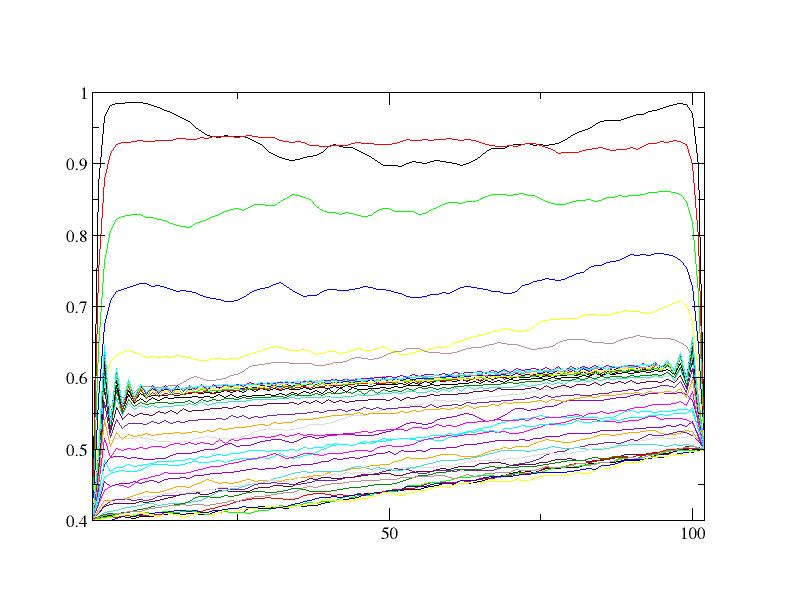
\includegraphics[width=0.5\linewidth]{profile.jpg}
\end{center}
    \vspace{-0em}
\caption{\label{fig:DenProfile} [Placeholder] Density profile for
  range of $\lambda$ from 0-100, with boundary conditions (0.5, 0.4) }
\end{figure}

\begin{figure}[h!]
\vspace{1em}
\begin{center}
% \begin{tabular}{c|c}
%    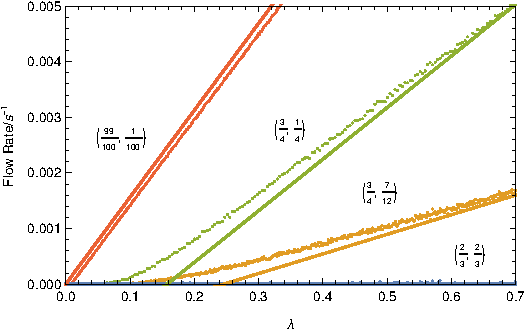
\includegraphics[width=0.5\linewidth]{newFlowMean.pdf} & 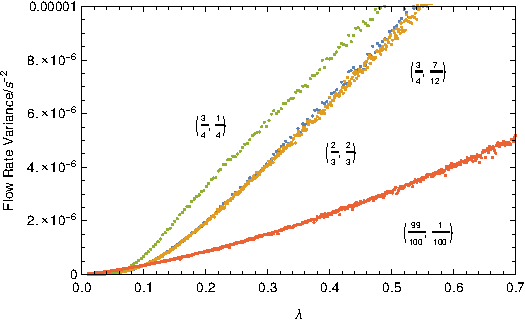
\includegraphics[width=0.5\linewidth]{newFlowVar.pdf} \\
%    \hline
%    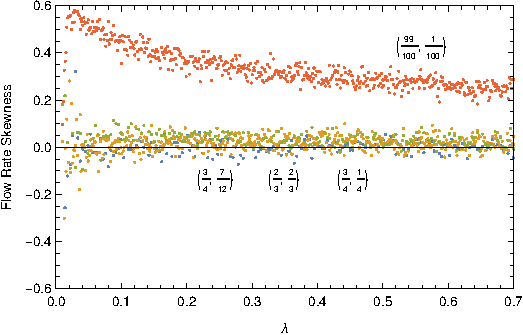
\includegraphics[width=0.5\linewidth]{newFlowSkew.pdf} & 
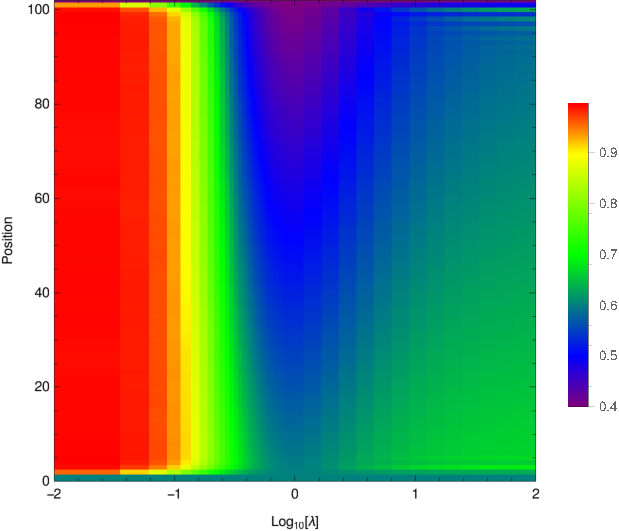
\includegraphics[width=0.5\linewidth]{graemeDensityProfile.pdf}
% \\
%    \end{tabular}
\end{center}
    \vspace{-0em}
\caption{\label{fig:flowStats} [Placeholder] Mean density within the flowing system as a function of stickiness for various boundary conditions.   
}
\end{figure}


\subsection{Review of the simulations}

Simulation of the sticky particle model reveals a number of curious
and unexpected features which have no equivalent in either SEP or the
1D Ising model.

\begin{itemize} \item 
A transition in flow character from $\lambda$ to $\lambda^4$.  
\item
The mean density of the system  has complicated variation with  $\lambda^4$.  
\item 
The effective diffusion constant has an extremum value at
  intermediate boundary density.
\end{itemize}

To get further understanding of these behaviours, we tackle the system
analytically.

\section{Mean Field Theory for Flow}
  
Let the spacing between lattice
sites be $a$, let $\tau_0$ be the free-particle hopping timescale, and
the time-averaged (or ensemble-averaged, assuming ergodicity)
occupation probability of the $i^{\mathrm{th}}$ lattice site be
$\rho_i$.  We will introduce $\zeta = 1 - \lambda $ here for convenience.

\subsubsection{Fokker-Planck Equation} Let the ensemble-averaged occupation
probability of the $i^\mathrm{th}$ site at time $t$ be $\rho_i
(t)$. In the mean-field approximation this is assumed to be
independent of $\rho_j(t)$ for $j \neq i $ at equal times. Therefore,
if the $i^\mathrm{th}$ site is occupied, then the rate at which it empties
is the sum of contributions from the
four permutations of the $(i+1)^\mathrm{th}$ and
$(i-1)^\mathrm{th}$ occupancy: 

\begin{align}
\begin{split}
 &\frac{1}{\tau_0 } (1-\rho_{i-1})\left[ (1 - \rho_{i+1}) + \lambda \rho_{i+1} \right] \\
 +&\frac{1}{\tau_0 } (1-\rho_{i+1})\left[ (1 - \rho_{i-1}) + \lambda \rho_{i-1} \right] .
\end{split}
 \end{align}

Similarly, if the $(i)^\mathrm{th}$ site is unoccupied, it fills with
rate which depends on the occupation probability of the neighbours,
and whether they are stuck to the $(i+2)^\mathrm{th}$ and $(i-2)^\mathrm{th}$ sites
respectively. Therefore, an unoccupied $i^\mathrm{th}$ site fills with rate
\begin{equation}
\frac{1}{\tau_0 } \left\{ \rho_{i+1} \left[ \lambda \rho_{i+2} + (1-\rho_{i+2}) \right] + \rho_{i-1} \left[ \lambda \rho_{i-2} + (1-\rho_{i-2}) \right] \right\}.
\end{equation}

If we now multiply the filling/emptying rates of site $i$ by the
probablity of being empty/full respectively, we obtain the
final Fokker-Planck equation for the site occupaution 

\begin{align}
\label{eq:latticeMFT}
\begin{split}
 \tau_0 \partDeriv{\rho_i}{t} &= \left( 1-\rho_i \right) \left[ \left(1-\zeta\rho_{i-2} \right) \rho_{i-1} + \left(1-\zeta\rho_{i+2} \right) \rho_{i+1} \right] \\
 &- \rho_i \left[ 2 \zeta \rho_{i-1} \rho_{i+1}  - (3-\zeta)\left(\rho_{i-1} + \rho_{i+1}\right) + 2 \right].
 \end{split}
 \end{align}


\subsubsection{Diffusion Equation: MFT Continuum Limit}
 To obtain the continuum limit of the MFT we substitute $\rho_i(t)
 \rightarrow \rho(x, t)$, $\rho_{i+m}(t) \rightarrow \rho(x + am, t)$
 into Eq.~\ref{eq:latticeMFT}.  Then, using a Taylor expansion around $x$ for
 small $a$, neglecting terms of $\mathcal{O}(a^4)$, and collecting
 terms we find that
\begin{align}
 \begin{split}
  \tau_0 \partDeriv{\rho}{t} =& a^2 \left[ 1-\zeta \rho (4-3\rho)  \right] \partDeriv{^2 \rho}{x^2} 
\\
  +& 2 a^2 \zeta (3\rho-2) \left(\partDeriv{\rho}{x}\right)^2 + \mathcal{O}(a^4) ,
 \end{split}
\end{align}
which can be factorized into the more familiar form of a continuity equation
\begin{equation}
\label{eq:contPDE}
 \partDeriv{\rho}{t} = \frac{a^2}{\tau_0} \partDeriv{}{x} \left\{ \left[1 - \zeta \rho\left(4-3\rho\right) \right] \partDeriv{\rho}{x} \right\},
\end{equation}
having dropped the higher-order terms.  From this we can identify the
flow $J(x)$ as the term in the curly brackets, and define a mean field
diffusion constant (see Fig.\ref{fig:diffCoef}):

\begin{equation} D_{MFT}(\zeta,\rho) =  \frac{a^2}{\tau_0} \left[ 1 - \zeta \rho\left(4-3\rho\right) \right ] \label{eq:diffCoef} \end{equation}

We note that the MFT diffusion constant can become negative. 
The density at
which this occurs is given by solving Eq.\ref{eq:diffCoef}:

\[\rho_c=\frac{2}{3} \pm \frac{1}{3} \sqrt(4-3/\zeta)\]

This has no real solution for $\zeta<0.75$.  So in the limit
of very sticky particles ($\lambda<0.25$) the MFT predicts a
transition between forward and backwards diffusion at some densities.  


\subsubsection{Limiting Cases}

In order to understand the implications of the MFT, let us consider
some limits. As $\zeta \rightarrow 0$ (i.e. as the model becomes a
simple exclusion model), $D \rightarrow \frac{a^2}{\tau_0}$. Likewise,
in the dilute limit $\rho \rightarrow 0$, $D \rightarrow \frac{
  a^2}{\tau_0}$, reflecting the fact that it becomes a dilute lattice
gas and therefore the interactions between particles become irrelevant
as they never meet.  Conversely, in the full limit $\rho \rightarrow
1$, $D \rightarrow \frac{\lambda a^2}{\tau_0}$; this is because we now
have a dilute gas of vacancies, which hop with rate
$\frac{\lambda}{\tau_0}$.  

One may observe that the 
MFT has a symmetry under $\rho \mapsto \frac{4}{3} - \rho$; thus, the
dynamics should be symmetric under a density profile reflection around
$\rho = \frac{2}{3}$. This is where $D$ always attains its extremal
value, $ \frac{a^2}{\tau_0}\left[1 - \frac{4}{3}\zeta\right]$, hence
for $\zeta>3/4$ the diffusion coefficient becomes negative in regions
with $\frac{2}{3} - \frac{\sqrt{\zeta\left(4\zeta - 3\right)}}{3\zeta}
< \rho < \frac{2}{3} + \frac{\sqrt{\zeta\left(4\zeta -
    3\right)}}{3\zeta}$. 

Finally, it is possible to show that
solutions to the continuum MFT containing domains with a negative
diffusion coefficient are linearly unstable; thus, if we try to have a
flow containing $\rho$ for which $D(\rho)<0$, the density of the
medium should gravitate towards one of the two densities for which $D(\rho)\sim
0$. Instead of observing ``backwards diffusion'' we would see an
extremely slow flow or no flow at all. 

\subsubsection{Steady State Flow}

It is possible to solve the continuum MFT in a steady state on a
finite domain, say $x\in(0, L)$. Steady state implies that there is no
build-up of particles $\partDeriv{\rho}{t}=0$, so the flow is constant through the system.

Using the constant-flow requirement for continuity
$J(x)=J_0=\mathrm{const.}$, and by integrating both sides of
equation\ref{eq:contPDE} with respect to $x$ we find that:

\begin{eqnarray}
 \int_{x_0}^x J(x')dx' &=& -\frac{a^2}{\tau_0} \int \! \! \mathrm{d} \rho \left[1 - \zeta
   \rho\left(4-3\rho\right) \right]\\ (x-x_0)J_0 & = & -\frac{a^2}{\tau_0}\left[ \rho + \zeta (\rho -
 2) \rho^2 \right ]
\label{eq:rho_x}
\end{eqnarray}

The density profile across the system is given by solving for
$\rho(x)$.  Since Eq.\ref{eq:rho_x} is cubic, the solution for density
$\rho(x)$ is non-unique for cases of high $\zeta$.  Thus in the limit of
high stickiness, the MFT is unable to make a unique prediction for the
density.  Furthermore, except in the SEP case $\zeta=0$, the density
will not vary linearly across the system.

\subsubsection{Dirichlet Boundary Conditions}

The constants $x_0$ and $J_0$ are the boundary conditions for the
flow, but they need not correspond to a physically-realisable
situation.  For driven systems it is more convenient to consider fixing
the density at each end. 

If we impose such Dirichlet boundary conditions on this system, say
$\rho(0)=\rho_0$ and $\rho(L)=\rho_L$, we find that
\begin{equation}\label{eq:MFTflow}
 J_0 = \frac{a^2}{L \tau_0} \left[ \rho_0 - \rho_L + \zeta \left( \rho_0\left[\rho_0^2-2\right] - \rho_L\left[\rho_L^2-2\right] \right) \right].
\end{equation}

This equation can be used for direct comparison with the simulations
(Figs.\ref{fig:constDens},\ref{fig:diffCoef}.  In general, the agreement is
good, except for the region where the MFT predicts negative flow.


\subsubsection{Interpretation of MFT}

The mean field theory enables us to predict flow behaviour of the MFT.
It recovers well-known limiting cases such as SEP ($\lambda=0$),
however at high stickiness ($\lambda<0.25$) it predicts its own
demise, with unphysical negative diffusion constants and by having
multiple solutions for the density at some positions in the system.
Moreover, at these conditions, the MFT does not give a unique density
profile.  This breakdown of the MFT corresponds to the transition to
slow flow observed in the simulation.

In some
conditions MFT predicts densities greater than 1.  One might guess that when the
MFT offers two possible values for the density, it will correspond to
a phase separation transformation in the actual system. Furthermore,
the MFT prediction of a maximum diffusion constant at a density of
$\rho=2/3$ suggests that this value of $\rho$ might be favoured for
strongly driven flows.

A curious feature of the MFT diffusion (Fig. \ref{fig:diffCoef}) is
that for fixed stickiness there are {\it two possible densities}
giving the same diffusion constant.  Thus it is possible to have a
steady state flow with phase separation into regions of high and low
density. This echoes the situation seen in short time-averages of the
simulation (Fig.\ref{fig:flowPatterns}) where blocks of high and low
density are evident.

Regarding the phase transition, we should note that we only have an
MFT prediction for the flow rate as a function of $\lambda$, since
$\rho(x)$ stops being unique when $\lambda$ drops below $\frac{1}{4}$,
and so the MFT lacks predictive power. For low-stickiness, when
$\lambda>\frac{1}{4}$, the MFT is in very good agreement with the
simulations, and this continues as $\lambda$ stretches into the
thousands, where the mean flow varies as $\mathcal{O}(\lambda^1)$.



\begin{figure}[h!]
\vspace{1em}
\begin{center}
 \begin{tabular}{c}
    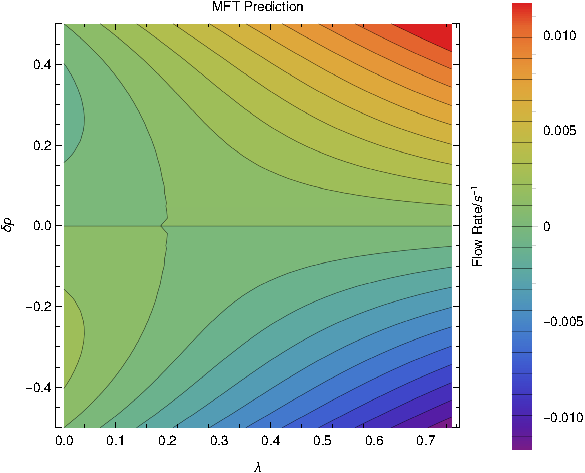
\includegraphics[width=0.48\linewidth]{newMftPred} 
    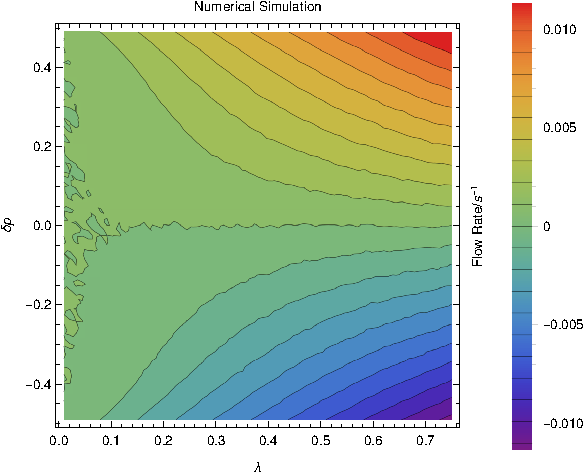
\includegraphics[width=0.48\linewidth]{newFlow}
    \end{tabular}
\end{center}
    \vspace{-2.5em}
\caption{\label{fig:constDens} Flow rate mean observed when varying the difference $\delta\rho$ between the boundary concentrations
$(\rho_0, \rho_L) = (\rho_M + \frac{1}{2} \delta\rho, \rho_M - \frac{1}{2} \delta\rho)$ and $\lambda$ (The top panel is the MFT prediction
for the flow rate, whilst bottom shows the observed mean flow rate).
We chose $\rho_M=\frac{1}{2}$, as this gives us the biggest range of $\delta\rho$ to investigate.
These calculations were performed with the same run parameters (system length etc) as above.
The MFT prediction (Fig.\ref{fig:constDens}a) shows a region of
negative flow - this occurs at $\zeta > \frac{4}{5}$ for the weakest
driving force, with additional stickiness required when the driving
force increases. The simulation exhibits close to zero flow in that
region (Fig.\ref{fig:constDens}b).  Away from this region, the MFT and
the simulation are in good agreement.
}
\end{figure}
The MFT prediction for the mean flow is again a good fit until $\lambda$ becomes sufficiently small,
and as before the simulations show no evidence of negative diffusion; rather the flow becomes critically slow for very sticky particles.
The higher moments of the flow (e.g. variance) do not show peaks, indicating that hard transitions are not occurring.
Finally, the density is very close to the average of the boundary densities until $\lambda$ drops below 1/4, at which point the system fills.

Continuing to specify the boundary densities to be $(\rho_0, \rho_L) = (\rho_M + \frac{1}{2} \delta\rho, \rho_M - \frac{1}{2} \delta\rho)$ for some given $\rho_M$, we can keep $\delta\rho$ relatively small, so that $J$ varies approximately
linearly with $\delta\rho$; thus if we calculate $J$ for a series of small $\delta \rho$, we can perform linear regression to find $D_\mathrm{Eff}=\partDeriv{J}{\delta\rho}\big|_{\delta\rho=0}$, the effective diffusion coefficient.
Computing this for different $(\rho_M, \lambda)$ combinations yields results that can be compared with Eq.~\ref{eq:MFTflow}.
\begin{figure}[h!]
\vspace{1em}
\begin{center}
 \begin{tabular}{c}
    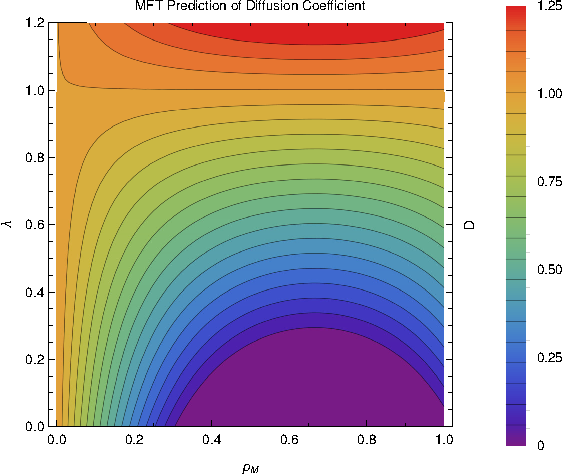
\includegraphics[width=0.48\linewidth]{newAnalFlow}
    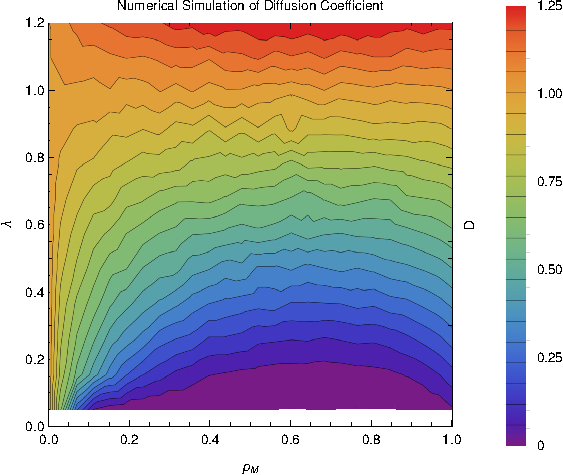
\includegraphics[width=0.48\linewidth]{newDataFlow}
    \end{tabular}
\end{center}
\caption{\label{fig:diffCoef}
Comparison of effective diffusion coefficient $D$ in the MFT (top) and in direct simulation (bottom) as a function of density and stickiness.
The white region is where the MFT gives negative diffusion. The simulations used 124 sites averaged over $\sim 10^9$ steps at each of $12 \times 24 \times 16 $ $(\lambda, \rho_M, \delta \rho)$ combinations.  
Full details in the supplementary materials.}
    \vspace{-2em}
\end{figure}

We compare the MFT prediction and the actual numerical results for the
diffusion constant in Fig.~\ref{fig:diffCoef}. We see that MFT and
simulation agree well for low stickiness, and both show the symmetry
about $\rho_M = \frac{2}{3}$. For high stickiness, where the MFT
prediction gives negative diffusion constant, we once again see low
positive values for the current.  It should be noted that the MFT
assumes that $\rho = \rho_M$ throughout, whereas in the simulations $\rho$ tends to be much higher.

It is instructive to get an overview of how the particles move during
flow. Fig.~\ref{fig:flowPatterns} show a plot of the flow structure in
the slow-flow regime.  In very short time averages the ``striped''
pattern indicates separation into dense and sparse regions, with an
overall concentration gradient arising from the relative size of such
regions.  Particle/vacancy diffusion through the empty/full regions
can be seen.  As the averages are taken over longer times the blocks themselves appear to diffuse.  Averaged over the entire simulation (not shown) the averaging simply gives a smooth density gradient.


Interesting structure is visible, the dynamics appearing as a random walk with
some tendency for particles to clump; over longer timescales the
diffusive behavior is more evident, with a textured structure
suggesting characteristic velocity of particles or vacancies through
emergent correlated clumps.  Additional plots can be found in the
supplementary materials.

\begin{figure}[h!]
\caption{\label{fig:flowPatterns} 
Indicative spacetime flow pattern for sticky free-flow $\left[\lambda = \frac{3}{20}, (\rho_0, \rho_L) = (\frac{3}{4}, \frac{1}{4})\right]$; other combinations shown in the supplementary materials.
Time runs along the x-axis, space (1 pixel=1 site) along the y-axis, with grayscale tone (black being empty, white being full) illustrating average site occupation over (clockwise from top left) $\frac{1}{32}$, $1$, $8$ and $32$ Gillespie steps per site respectively.}
\begin{center}
 \begin{tabular}{c | c}
    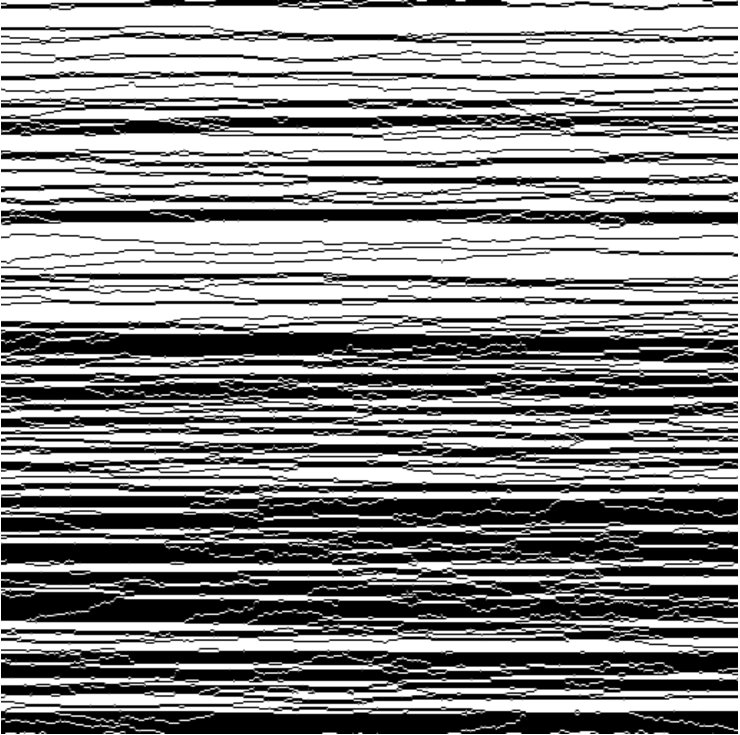
\includegraphics[width=0.49\linewidth]{shortTime}  &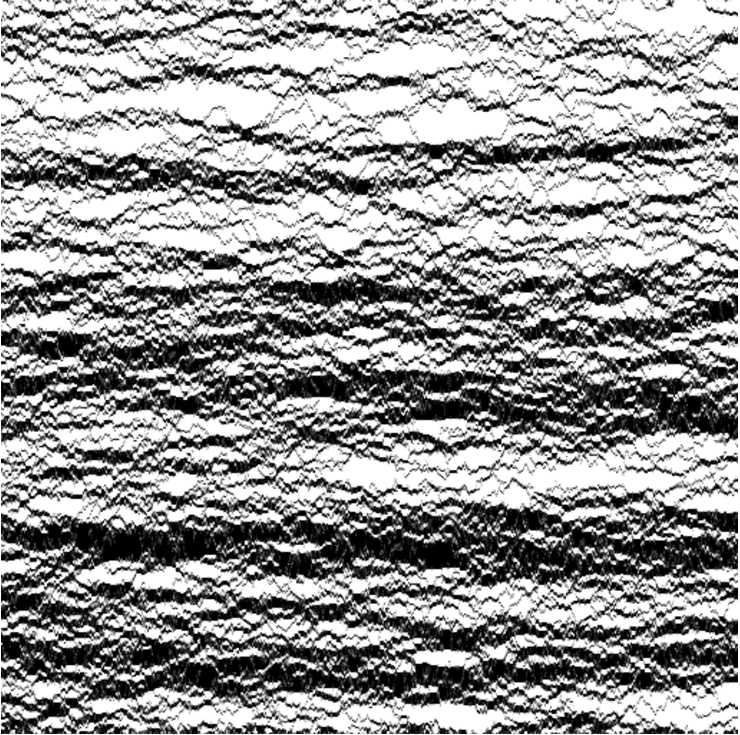
\includegraphics[width=0.49\linewidth]{midShortTime} \\
    \hline
    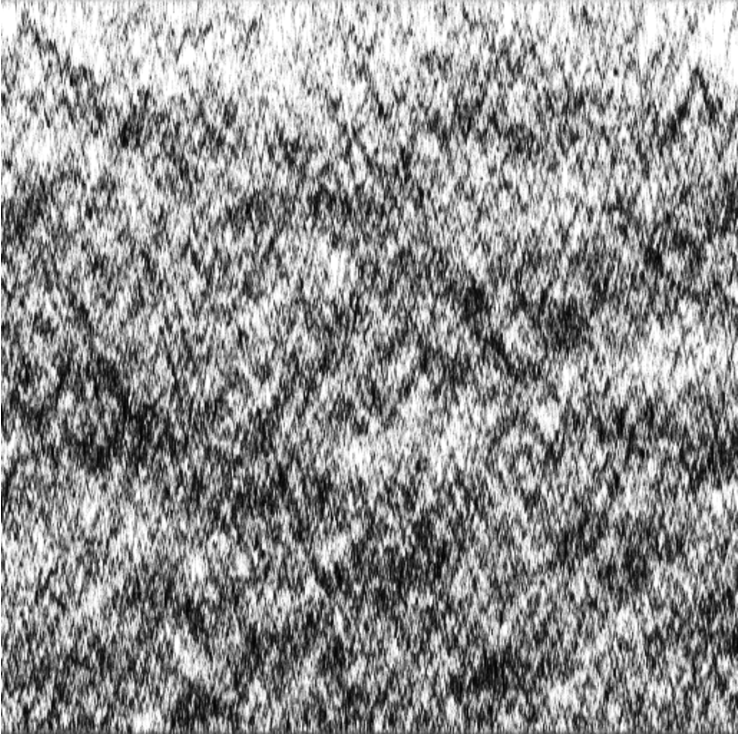
\includegraphics[width=0.49\linewidth]{longTime} &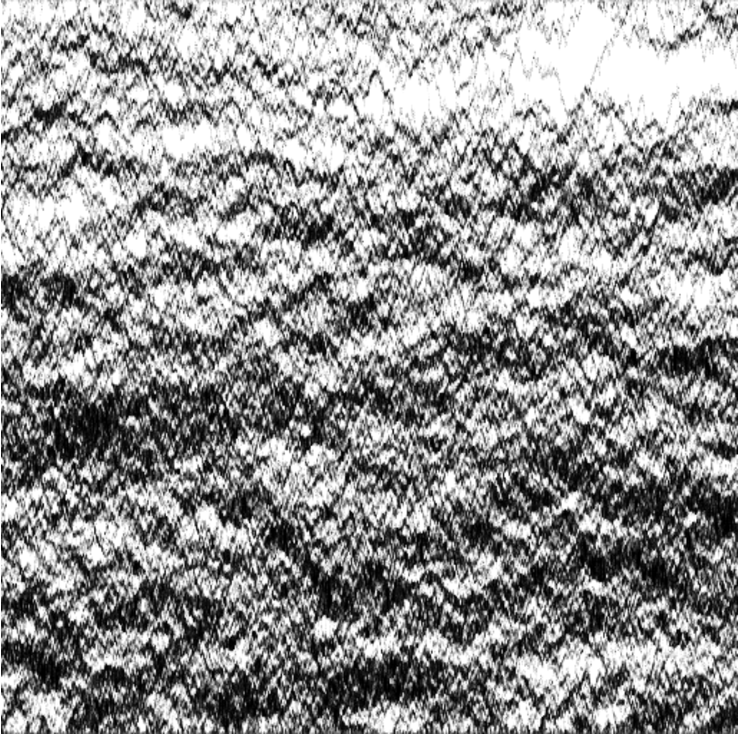
\includegraphics[width=0.49\linewidth]{midLongTime}
    \end{tabular}
\end{center}
    \vspace{-2em}
\end{figure}

\section{Discussion and conclusions}

The sticky particle model is the combination of the Ising model with
symmetric exclusion process.  It arguably represents the simplest
possible flow model for interacting particles is a homogeneous medium.

Although only the particles exhibit
stickiness, the analytics suggest a symmetry between vacancy-type and
particle-type flow at density of $\frac{2}{3}$, which is observed in
the simulation.  The flow exhibits a foamy pattern with intermediate
time-and-space correlations.  The continuum solution MFT is a good
predictor of the bulk flow behavior of the SPM.  The negative
diffusion constant found in MFT at high stickiness indicates that the
assumption of homogeneous density break down: thus the MFT predicts
its own demise, and this agrees well with our numerics.

Above a certain level of stickiness, the model exhibits a
nonequilibrium phase transition to a slow-flowing phase.  The require
stickiness for the transition is dependent on the strength of the
driving force - a strongly driven system inhibits the flow.  Mean field
analysis, together with visualization of the flowing system, suggest
that the transition comes when the density becomes inhomogeneous.

A number of questions remain open. Is there a physical principle which
determines the density?  Why does the strongly repelling system
produce a density with maximum flow?  Can one derive the $~\lambda^4$
dependence of the slow-flow?

\section*{Acknowledgements}
We would like to thank EPSRC (student grant 1527137) and Wolfson
Foundation and ERC for providing funding, Mikael Leetmaa for producing
\texttt{KMCLib}, and the \texttt{Eddie3} team here at Edinburgh for
maintaining the hardware used.  We would also like to thank Martin
Evans, Bartek Waclaw and Richard Blythe for some very helpful
discussions.

\bibliography{jHellStickyParticleMain}



\end{document}
%
% ****** End of file apssamp.tex ******
